\section{LSTM}
LSTM (abbreviation for Long-short Term Memory) is a variant of recurrent neural network. LSTM seeks to solve vanishing gradient and exploding gradient problem in vanilla recurrent neural network. These problems happen when a training sequence is too long. LSTM introduces gating concept in recurrent neural network. An LSTM contains three gates, an input gate, an output gate, and a forget gate. A forget gate determines when to reset the content of the cell memory. An input and output gate control the flows of input and output of the LSTM respectively.
\begin{figure}[h]
	\centering
	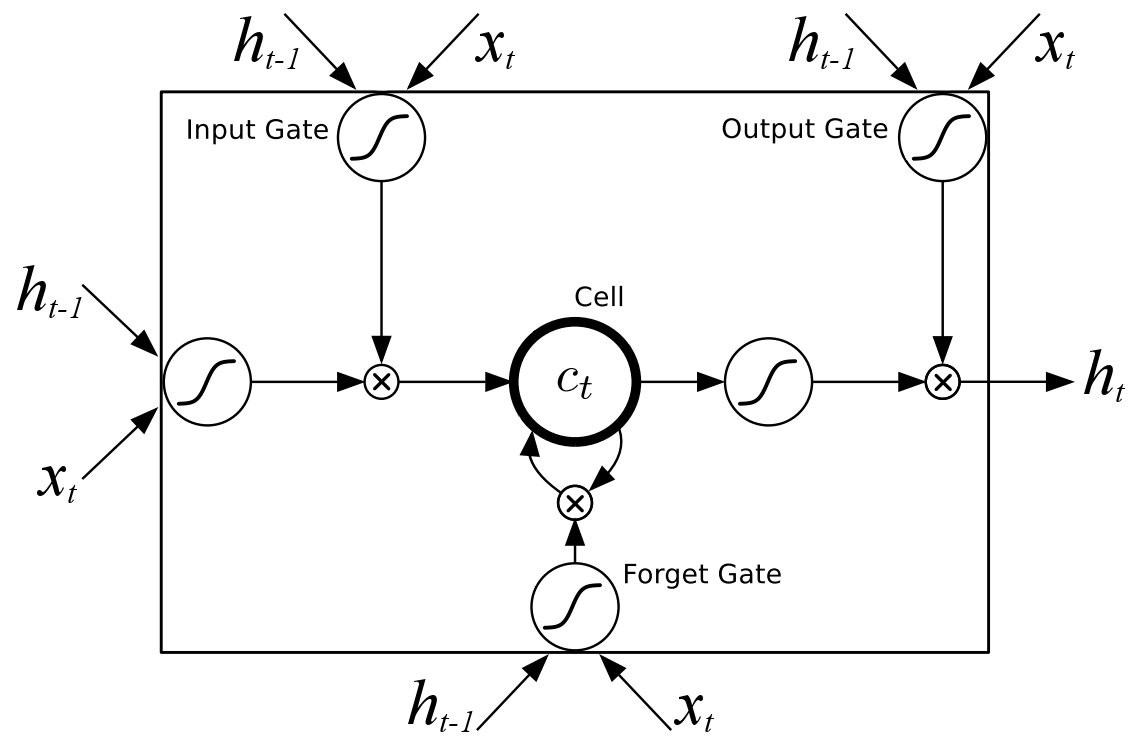
\includegraphics[width=0.85 \textwidth]{assets/lstm.png}
	\caption{An LSTM unit}
	\label{fig:lstm}
\end{figure} \\
We use LSTM unit provided by Caffe\footnote{\href{https://github.com/BVLC/caffe}{Caffe} is developed by Berkeley Vision and Learning Center (BVLC)} framework. It requires CUDA 8 and cuDNN v5.1 from Nvidia, which enable Caffe framework to utilize Nvidia GPU to train a neural network. We used Nvidia GTX 850m to train our LSTM model. This GPU is pretty decent to train a medium-sized network. \\ \\
